\subsection{Overview}

Our S\&C subsystem consists of :
\begin{itemize}
    \item Control Boards: 
    \begin{itemize}
            \item Braking Controller
            \item Thermal (Cooling) Controller
            \item Telemetry Controller
    \end{itemize}

    \item Telemetry Device: 
    \begin{itemize}
            \item CAN Bus
            \item Telemetry Transceiver
            \item Network Transceiver
            \item GUI/Logging system
    \end{itemize}
\end{itemize}
In this section, the main components of the sensor network and software architecture shall be described, as well as their basic functionality. A special focus shall be made on how safety mechanisms are implemented in these systems. Extensive design descriptions are expected for, if applicable:

\subsection{Control Boards}
\subsubsection{Introduction}
    Overview of all control boards (Brakes, Thermal, Telemetry):
    \begin{itemize}
        \item Brakes Controller: \\
        The brakes board controls the pod's friction braking system.
        It drives the solenoid valves that are connected to the braking mechanisms.
        The board's design engage the brakes by default for safety, releasing them only when all safety criteria are met,
        which come from the sensors and user commands. 
        It utilizes a Texas Instrument C2000 series microcontroller.
        \item Thermal (Cooling) Controller: The thermal board drives the coolant pump via a PWM to a MOSFET bridge, adjusting the pump speed based on the feedback from temperature and flowrate sensors in the cooling loop.
        The system design also includes continuous monitoring of temperatures at multiple (critical) areas of the Fermion to detect overheating. 
        \item Telemetry Controller: The telemetry board is the pod's communication system, facilitating bidirectional data exchange between the pod and the user device, typically a laptop.
        It is responsible for sending commands to the pod and receiving diagnostic and sensor information in return.
        The system uses the CAN bus for communication in the pod.
    \end{itemize}
  
Our Sense\&Control system includes three main boards: \\
For the Braking Managament System \textbf{TO BE ADDED} \\
The Thermal Management Controller is responsible for cooling the Traction Components, i.e., Motor and Traction Controller. The actuator is the coolant pump which is controlled  with the feedback of the temperature of coolant in the cooling loop (Refer to Diagram for Visualisation).  The Pump Speed is controlled via PWM to the MOSFET Bridge. The PWM duty cycle is simply calculated from a lookup table that is referenced to the temperature difference between target and actual temperatures. The only safety feature to be developed is to issue an emergency stop signal to HV Systems in the event the coolant temperature exceeds a critical temperature. \\
Finally, the Telemetry Unit is responsible for receiving commands from, and transmitting diagnostic and sensor information to the commanding PC. The Telemetry unit then receives and broadcasts information as well as commands on the CAN bus as a Master Controller to all the slave devices. \\
Diagram with the connection of all boards with NAP and control station:

%Für Ian: Das ist als Netzwerkdiagramm gedacht. Einfach telemetrysystems.png nehmen, ggf. kennzeichnen was unser NAP und control station ist. Das unten kommt erst später-
%DINO: Check this information
The telemetry system connects to a Network Access Point, which is the Rocket M2 as proposed by EHW. It transfers to the control station, which will be a team member's commanding PC (user device).
\begin{figure}[H]
    \centering
    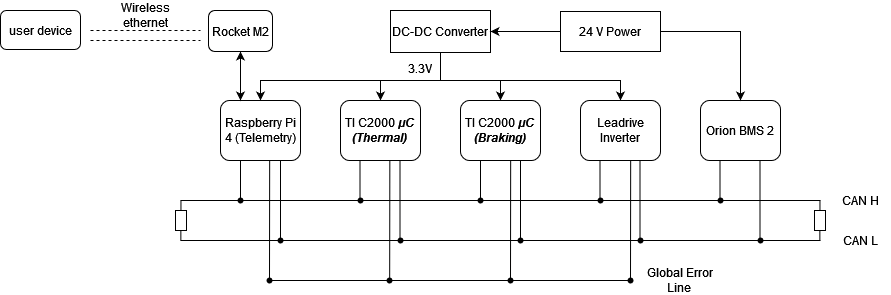
\includegraphics[width=\textwidth]{texfiles/elec/eimg/telemetrysystems.png}
    \caption{Overall Structure of the Telemetry System}
    \label{fig:enter-label}
\end{figure}

%DINO: Added (Networks) down there thought just hardware might be confusing. If it makes sense, erase the ()
The implementation of the  hardware architecture goes as follows: 

% FÜR IAN: habe hier aktuelle graphiken eingefügt, beschriftungen angepasst. musst du halt irgendwo an die richtige stelle schieben. schau mal was begin{figure}[h] macht.:
%Done. Einfach H in alle gemacht. So sieht's gut genug 

    \begin{figure}[H]
        \centering
        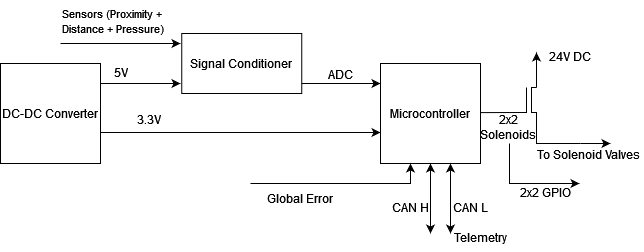
\includegraphics[width=0.9\linewidth]{texfiles/elec/eimg/Brakesystems}
        \caption{Brakes Controller Schematic} 
        \label{fig:Brakes Controller Schematic}
    \end{figure}
 \begin{figure}[H]
        \centering
        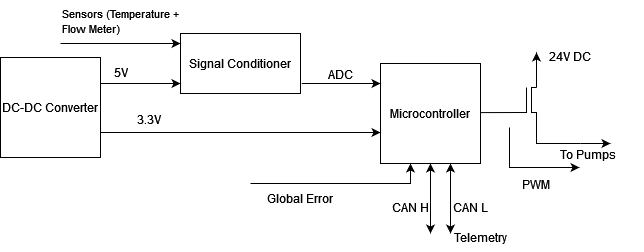
\includegraphics[width=0.9\linewidth]{texfiles/elec/eimg/thermalsystems}
        \caption{Thermal Controller Schematic}
        \label{fig:Thermal Controller Schematic}
    \end{figure}
 \begin{figure}[H]
        \centering
        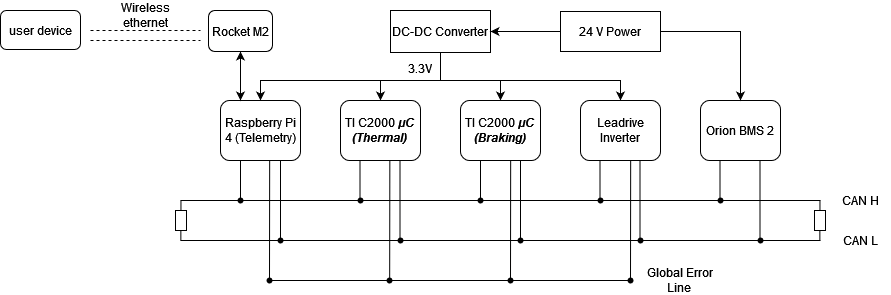
\includegraphics[width=0.9\textwidth]{texfiles/elec/eimg/telemetrysystems}
        \caption{Telemetry Unit Hardware Architecture}
        \label{fig:Telemetry Unit Hardware Architecture}
\end{figure}
Communication protocols used: 
\begin{itemize}
    \item Control Area Network (CAN): CAN was implemented as the inter-board communication protocol. This decision is inspired by the automotive industry, where CAN has been used for decades as a robust and physically reliable protocol.
    To add to that, many of our OEM devices (only) support CAN communication. \href{https://www.ti.com/lit/an/sloa101b/sloa101b.pdf}{CAN Description}.
    \item TCP/IP: Used to transmit data between the Telemetry Unit and command PC. We transmit wirelessly via UDP between the Rocket M2 and the command PC.
    
    \item Serial Peripheral Interface (SPI): Left empty on purpose.
    \begin{comment}
        Synchronous, full-duplex communication protocol used for connecting peripheral devices.The master device generates the clock signal on SCLK while transmitting data to the slave device via MOSI, and the slave device responds with data on MISO. Communication occurs simultaneously in both directions, what allows high-speed data transfer between devices \footnote{\href{https://www.ti.com/lit/ug/sprugp2a/sprugp2a.pdf?ts=1710046776474\}{SPI Description}}.
    \end{comment}
    \item Inter-Integrated Circuit (I2C): Multi-device communication protocol used for connecting sensors. Uses Master-Slave-Architecture.
\end{itemize}

\begin{comment}

    \begin{itemize}
            \item Control Area Network (CAN): CAN was implemented as the inter-board communication protocol. This decision is inspired by the automotive industry, where CAN has been used for decades as a robust and physically reliable protocol.
            To add to that, many of our OEM devices (only) support CAN communication. \href{https://www.ti.com/lit/an/sloa101b/sloa101b.pdf}{CAN Description}.
            %Für IAN add Link to CAN Description online
            % DINO: I think you mean reference. Check if Footnote done correctly. Also did the same for SPI 
            \item TCP/IP: Used to transmit data between the Telemetry Unit and command PC. We transmit wirelessly via UDP between the Rocket M2 and the command PC.
            \item Serial Peripheral Interface (SPI): Synchronous, full-duplex communication protocol used for connecting peripheral devices.The master device generates the clock signal on SCLK while transmitting data to the slave device via MOSI, and the slave device responds with data on MISO. Communication occurs simultaneously in both directions, what allows high-speed data transfer between devices \footnote{\href{https://www.ti.com/lit/ug/sprugp2a/sprugp2a.pdf?ts=1710046776474\}{SPI Description}}.
            \item Inter-Integrated Circuit (I2C): Multi-device communication protocol used for connecting sensors.
    \end{itemize}

\end{comment}
% Merged detailed content from the first snippet

\subsection{State Machine of the Vehicle}
% Continue with the structured format from the second snippet, ensuring to merge relevant content from the first snippet into these sections.

We use different states in each component.
Generally (and in the main control of the pod), we have the following structure of states:
\begin{figure}[H]
    \centering
   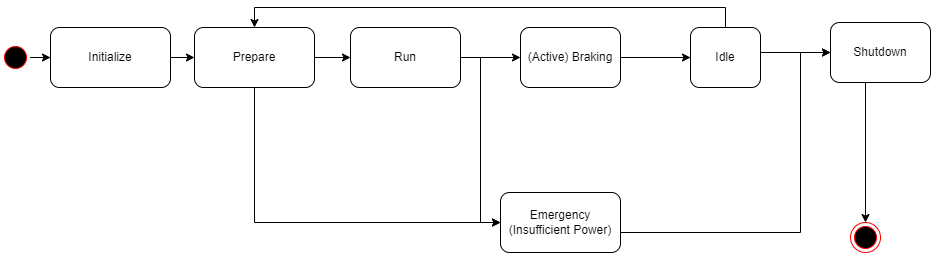
\includegraphics[width=0.9\textwidth]{texfiles/elec/eimg/Statechart}
    \caption{Overall State Chart}
    \label{fig:overall-state-chart}
\end{figure}
Because of layout reasons, we decided to give the transitions and actions seperately:
\begin{itemize}
    \item Transitions requires:
    \begin{itemize}
        \item Initialize:
        \begin{itemize}
            \item Prepare: When all systems have been powered on. Controllers automatically enter this state.
        \end{itemize}
        \item Prepare:
        \begin{itemize}
            \item Emergency: Run conditions not met, which may be
            \begin{itemize}
                \item Insufficient initial Brake Pressure
                \item Overheat
                \item IMD trigger
                \item Global Error Line Trigger
                \item Undervoltage
                \item Manual Interruption
            \end{itemize}
            \item Run: Prepare finished without incidents.
        \end{itemize}
        \item Run:
        \begin{itemize}
            \item Emergency: Safety hazard, such as
            \begin{itemize}
                \item Insufficient Brake Pressure/Pressure Leak
                \item Overheat
                \item IMD trigger
                \item Undervoltage
                \item Global Error Line Trigger
                \item Manual emergency
            \end{itemize}
        \end{itemize}
        \item Braking:
        \begin{itemize}
            \item Idle:
            \begin{itemize}
                \item Speed = Zero
            \end{itemize}
        \end{itemize}
        \item Idle:
        \begin{itemize}
            \item Prepare:
            \begin{itemize}
                \item Manual decision
                \item Requires: No emergency condition
            \end{itemize}
            \item Shutdown:
            \begin{itemize}
                \item DC Link almost discharged
                \item Speed = Zero
            \end{itemize}
        \end{itemize}
        \item Emergency:
        \begin{itemize}
            \item Shutdown:
            \begin{itemize}
                \item Safe shutdown conditions
                \item DC Link almost discharged
                \item Speed = Zero
            \end{itemize}
        \end{itemize}
    \end{itemize}
\end{itemize}

\subsection{Code Architecture and Class Diagram}
% Insert content from the first snippet related to Code Architecture here.
For each system respectively was the following software architecture implemented: Concerning the rulebook, we point out that the brakes controller checks for air pressure before and during running, while the thermal system checks for overtemperature, especially when temperatures are increasing. However, our simulations show that this is very unlikely to happen.
\begin{figure}[H]
        \centering
       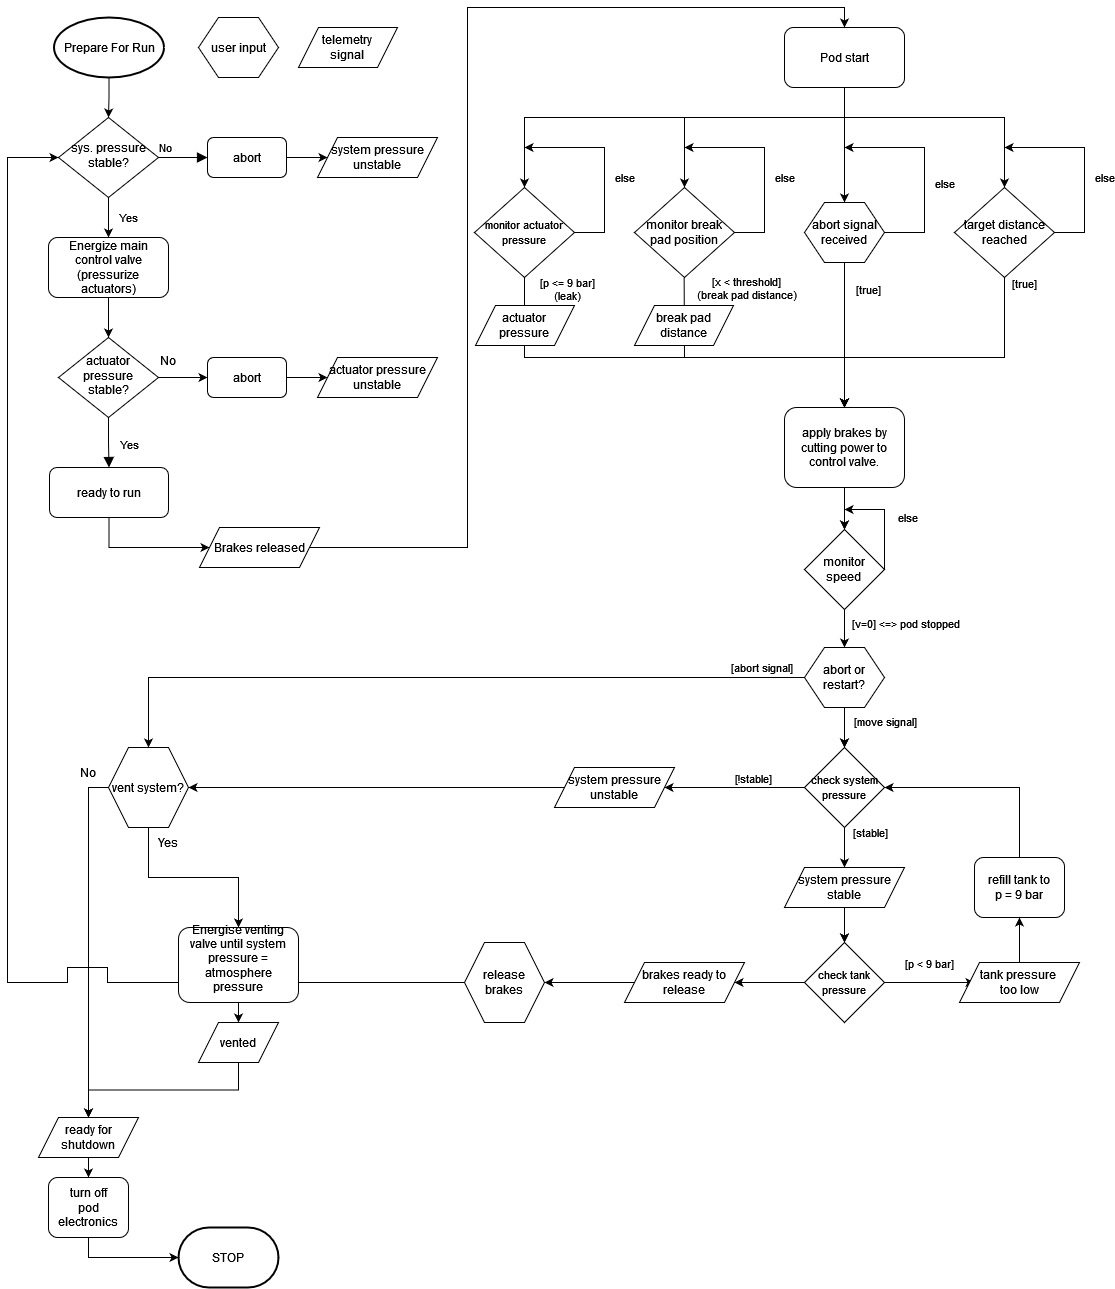
\includegraphics[width=\textwidth]{texfiles/elec/eimg/brakesoftware_ext}
        \caption{Brakes System Software Architecture}
        \label{fig:Brakes System Software Architecture}
    \end{figure}

\begin{figure}[H]
        \centering
       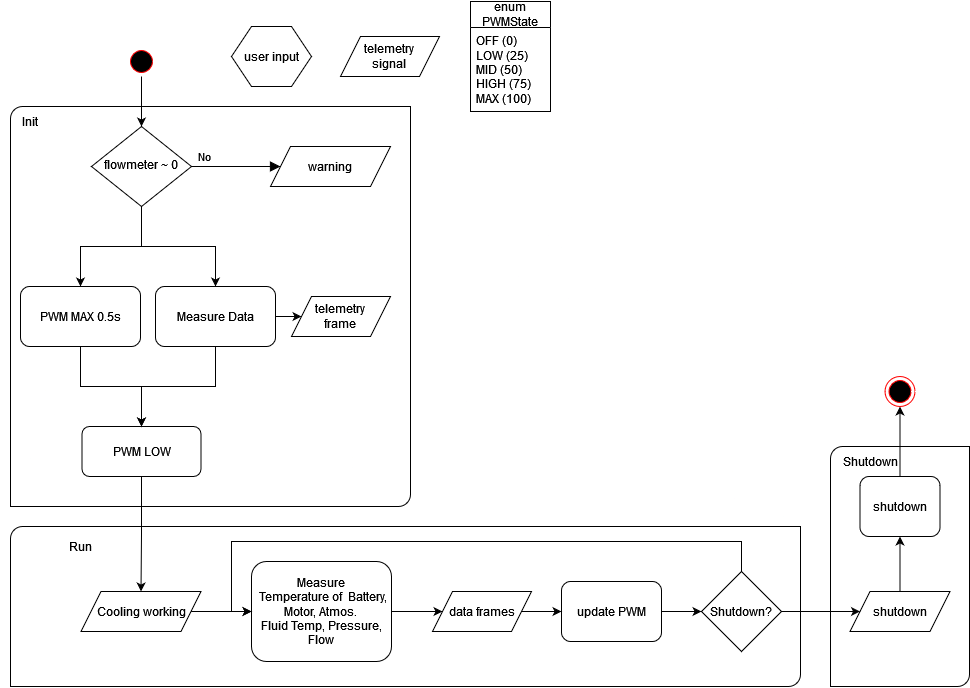
\includegraphics[width=\textwidth]{texfiles/elec/eimg/thermalsystemsflowchartsoftware}
        \caption{Thermal System Software Architecture}
        \label{fig:Thermal System Software Architecture}
    \end{figure}

\begin{figure}[H]
        \centering
       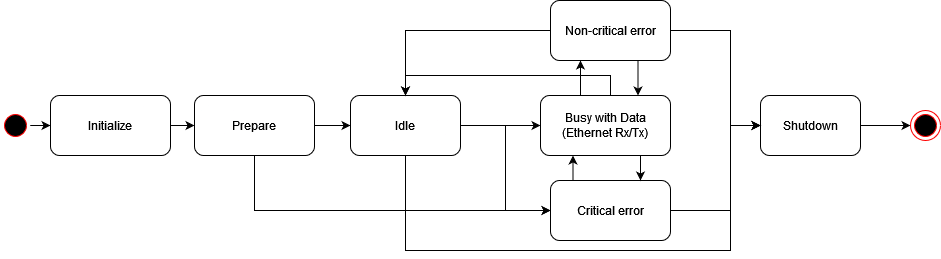
\includegraphics[width=\textwidth]{texfiles/elec/eimg/telemetrystate.png}
        \caption{Telemetry Unit Software Architecture}
        \label{fig:Telemetry Unit Software Architecture}
    \end{figure}

\subsection{Control Boards/Units in the Vehicle}
% Insert content from the first snippet related to Control Boards/Units in the Vehicle here.

\begin{enumerate}
    \item Brakes Controller
    \begin{enumerate}
        \item Requirements of the board.
        Parts List:
        \begin{table}[H]
            \centering
            \begin{adjustbox}{width=\textwidth,center}
                \begin{tabular}{|>{\bfseries}m{2cm}|m{4cm}|m{1.5cm}|m{1.5cm}|m{2cm}|m{2cm}|m{2cm}|}
                \hline
                Component & Company/Product Name & Quantity & Mass [kg] & Size [mm] & Producer & Nominal Voltage \\
                \hline
                NTC Thermistor & Vishay NTCLE413E2103F102L & x40 & 0.03 & 1000 x 3 x 3 & Outsourced & 500 \\
                \hline
                Coolant Pump & Pierburg & 1 & 1 & - & Sponsored & 12 \\
                Speed Sensor & Festo & x2 & 0.01 & - & Sponsored & 12 \\
                \hline
                \end{tabular}
            \end{adjustbox}
            \caption{Outline of Components of the Thermal Controller}
            \label{tab:thermal-ctrl-components}
        \end{table}
The complete part list can be found in \href{https://docs.google.com/spreadsheets/d/1GvvRlhKn8gMCE3rAxvrYHUjA288l9iqX/edit#gid=378650025}{this table}. \\

% DI: This table should completely go away now that we have the hyperlink. @IAN hyperlink is for the detailed ones. Left it in case you thought we should still use it This is a problematic URL\footnote{\href{https://www.ti.com/lit/ug/sprugp2a/sprugp2a.pdf}{Click here to open}}.

        \item Hardware Rationale (HW design and concerns). \\
        Critical points: Safety. The brakes should engage by default, and only release when all safety criteria are met. The board should be designed to be fail-safe, and process information and requests quickly.
        Our brakes controller's \href{https://drive.google.com/file/d/1a7zaJbmfFdLdrrGtLt2_ySVTqbc168NL/}{hardware design documentation} is uploaded (non-publicly) online, to view for the reader. We show only the schematic here. 
        \begin{figure}[H]
            \centering
            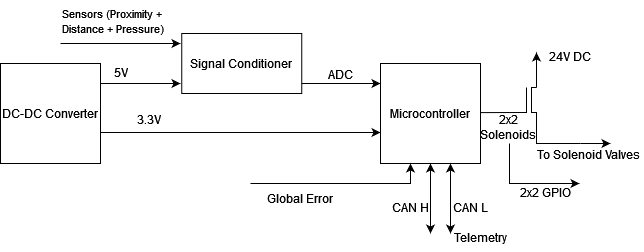
\includegraphics[width=0.7\linewidth]{texfiles/elec/eimg/Brakesystems}
            \caption{Brakes Controller Hardware Schematic}
            \label{fig:Brakes Controller Hardware Schematic}
        \end{figure}


        \item Firmware Rationale (Internal State machine and design concerns).
        No stuck loops. Real-life transport scenario: Re-release of brakes is possible. 
        %Für Ian zum ausformulieren.
        %DINO: ONly added int. machine. 


        What concerns the state flow of the system, it can be described as follows:
        \begin{figure}[H]
            \centering
            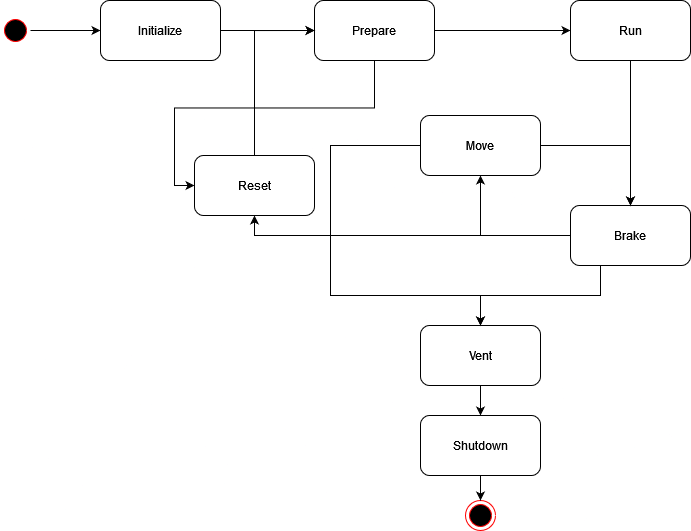
\includegraphics[width=0.6\linewidth]{texfiles/elec/eimg/BrakesStatechart.png}
            \caption{Brakes Controller Internal State Machine}
            \label{fig:Brakes stateflow}
        \end{figure}

        \item Testing and validation plan.


    \end{enumerate}

    \item Thermal Controller
        \begin{enumerate}
            \item Requirements of the board.\\
            Should drive the coolant pump. The control algorithm, planned as a PID controller, is to be implemented, but not necessary. We can let the thermal system run on a on-off scheme, which is less effective, but easier.

        \begin{table}[H]
            \centering
            \begin{adjustbox}{width=\textwidth,center}
            \begin{tabular}{|>{\bfseries}m{2cm}|m{4cm}|m{1.5cm}|m{1.5cm}|m{2cm}|m{2cm}|m{2cm}|}
                \hline
                Component & Company/Product Name & Quantity & Mass [kg] & Size [mm] & Producer & Nominal Voltage \\
                \hline
                Microcontroller & Texas Instruments F280039C & 1 & - & - & - & - \\
                \hline
                Multiplexer & Texas Instruments & 8 & - & - & - & - \\
                \hline
                NTC Thermistor & Vishay NTCLE413E2103F102L & x40 & 0.03 & 1000 x 3 x 3 & Outsourced & 500 \\
                \hline
                Coolant Pump & Pierburg & 1 & 1 & - & Sponsored & 12 \\
                Speed Sensor & Festo & x2 & 0.01 & - & Sponsored & 12 \\
                Heat Conductors Muster & Würth & 2 & - & - & - & - \\
                \hline
            \end{tabular}
            \end{adjustbox}
            \caption{Components of the Telemetry Controller}
            \label{tab:telemetry-ctrl-components}
        \end{table}
            \item Hardware Rationale (HW design and concerns).
            Simplicity. The brakes controller design was big. The thermal controller is mainly gathering sensor data, such as temperature sensors, and flow rate, and controlling the pump. The pump is a simple on-off device, and the (fine) temperature control is not critical. We set that 50 C shall not be exceeded in the batteries (which is not cooled by the liquid cooling system), while traction inverter and motor shall stay under 60 C. If we require a fan for the battery, it will be controlled by the BMS.
            \item Firmware Rationale (Internal State machine and design concerns).
            \item Testing and validation plan.
            \begin{itemize}
                \item Test maximum volume (mass transfer) power of pump.
                \item The temperature sensors should be tested for their accuracy and deviance.
                \item The control algorithm should be tested for its effectiveness, and delay due to mechanical and thermodynamical factors.
                \item Test flow system sensors for accuracy and deviance.
                \item Test maximum cooling power of pump. This testing scenario will not be used during the competition.
            \end{itemize}
    \end{enumerate}

        \item Telemetry Controller
        \begin{enumerate}
            \item Requirements of the board.
            Parts Lists
                \begin{table}[H]
                    \centering
                    \begin{tabular}{|c|c|c|}
                    \hline
                    \textbf{Part} & \textbf{Manufacturer} & \textbf{Description} \\ \hline
                    Raspberry Pi Zero 2 W & Raspberry & Microcontroller for telemetry \\ \hline
                    Raspberry Pi 4 B & Raspberry & Computer for telemetry \\ \hline
                    MC3479 & Memsic & 3-Axis Accelerometer \\ \hline
                    RS485 CAN HAT & Waveshare & CAN adapter for RPI4B \\ \hline
                    \end{tabular}
                    \caption{Telemetry System Parts List}
                    \label{tab:my-table}
                \end{table}
            \item Hardware Rationale (HW design and concerns).
            
            \item Firmware Rationale (Internal State machine and design concerns).
%To Ian: Include the state machines at Software Rationale.
%Di: check if correct. Mostly done with gpt. I think it did a great job doing the foundation though. 
%Did not do a great job
                The design concerns were:
                \begin{itemize}
                    \item Process data transmission from CAN line to the GUI in the user device. CAN bus simulations with CANoe have shown that the transmission speed is sufficient to not to stall the line. The data is transmitted more often than at 2 Hz.
                    \item Process command transmission to the CAN line from the GUI in the user device in less then 100ms. With measuring transmission speeds of ~10ms, this is not a concern.
                    \item The system should be able to handle the data from the sensors and the commands from the user.
                \end{itemize}
        The state flow of the thermal system can be described as such:
        \begin{figure}[H]
            \centering
            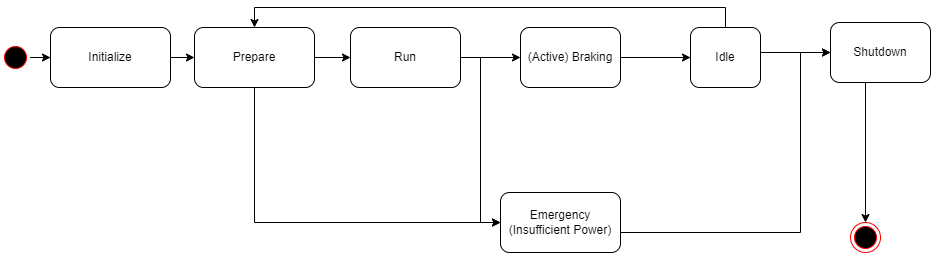
\includegraphics[width=0.7\linewidth]{texfiles/elec/eimg/ThermoStateflow.png}
            \caption{Thermal Controller Internal State Machine}
            \label{fig:Thermal stateflow}
        \end{figure}


            \item Testing and validation plan.
        \end{enumerate}
\end{enumerate}

\subsection{Communication and Navigation}
\subsubsection*{Communication}
For communication, we use our telemetry system, transmitting bidirectionally telemetry data and commands to the pod. The telemetry system uses the CAN bus, which is a robust and reliable protocol that will not be explained further, presuming that the reader is already familiar with it. \\
The VCU, in this sense, is a Raspberry Pi 4B, which is connected to the CAN bus via a RS485 CAN HAT. 
Through its connectivity abilities, we can connect to a Wireless LAN system for (necessary) remote control. We use the Rocket M2 as a transmitter. A short estimation of scales of speed between electromagnetic fields and the speed of common ground transportation modes show that we have not reached the speed where the Doppler effect of the signals play any significant role, so we do not take that into consideration. We use the open-source GUI system of Swissloop and plan to develop our own data logging system as an addition. The addition we plan to add to the GUI system are the following:
\begin{itemize}
    \item (Cosmetic) adaption to the Fermion, including \begin{itemize}
        \item the battery pack layout for both batteries
        \item the thermal system data
        \item acceleration data
        \item check for abnormal situations (out of range values) and carrying out safety procedures, consisting of:
        \begin{itemize}
            \item LV or HV Battery temperature or voltage out of range:
            \begin{itemize}
                \item Go into emergency state and shutdown
            \end{itemize}
            \item Temperature in motor or inverter close (10C) to operational limit:
            \begin{itemize}
                \item Set cooling pump to maximum. Limit current to inverter.
            \end{itemize}
            \item Temperature in motor or inverter over operational limit for more than 1 second:
            \begin{itemize}
                \item Assuming that previous state has been reached already, cut power to HV.
            \end{itemize}
            \item Brakes pressure out of range:
            \begin{itemize}
                \item To emergency.
            \end{itemize}
            \item Speed too high:
            \begin{itemize}
                \item Apply brakes.
            \end{itemize}
            \item IMD leak:
            \begin{itemize}
                \item To emergency. Proceed only with safety equipment (gloves, glasses, boots)
            \end{itemize}
            \item Latency of GUI too high/heartbeat missed:
            \begin{itemize}
                \item After second time: Emergency 
            \end{itemize}
        \end{itemize}
    \end{itemize}
    \item Time Counter since start of run
    \item More informative audiovisual feedback
\end{itemize} 

\subsubsection*{Navigation and Control}
Our navigation system does not incorporate railway-like switches, nor GPS due to the track's short length. Instead, the pod solely uses an accelerometer and speed sensors to measure the velocities of both the front (guiding) wheel and the back (propulsion) wheel,
determining the pod's dynamics. This also includes vibrations.\\
In this iteration, we have clearly defined competition rules, and hence stick to simple acceleration/velocity/distance curved. In the future, we plan to implement a more complex navigation system, including a system that can compute the acceleration/speed automatically, which is a more realistic use case. \\
Our sequence of the run is as follows:
\begin{itemize}
    \item Start sequence:
    \begin{itemize}
        \item Initialize:
        \begin{itemize}
            \item Start Telemetry System
            \item Start BMS
            \item Start Cooling System at 0% Pump Rate
            \item Start Braking System
            \item Send signal to GUI
        \end{itemize}
        \item Prepare:
        \begin{itemize}
            \item Start Inverter (KL30)
            \item Open precharge relay (~ 5s)
            \item Open HV relay
            \item Close precharge relay
            \item Every individual system checks preparations
        \end{itemize}
    \end{itemize}
    \item Run sequence:
    \begin{itemize}
        \item Start Cooling System at 50% Pump Rate
        \item Release Brakes
        \item Propel inverter to target speed
        \item Wait for errors or stop signal
    \end{itemize}
    \item Brake sequence = Decelerating = Emergency Braking:
    \begin{itemize}
        \item Open precharge relay and HV relay and open valves (with same signal)
        \item Wait until speed is zero
    \end{itemize}
    \item Shutdown sequence:
    \begin{itemize}
        \item HV relay is opened
        \item Check:
        \begin{itemize}
            \item Speed Zero
            \item Acceleration next to zero
            \item Brakes Vented
            \item Thermal Pump down
        \end{itemize}
        \item Inverter shuts down (Turnoff KL30)
        \item Brakes are shut down
        \item BMS is shut down
        \item Cooling system is shut down
        \item Telemetry system is shut down
    \end{itemize}
\end{itemize}

\subsubsection{Design requirements}
The Telemetry Devices possesses the following properties and constraints:
\begin{table}[H]
    \centering
    \begin{adjustbox}{width=0.5\textwidth,center}
    \begin{tabular}{|c|c|}
    \hline
        \textbf{Constraint/Specification} & \textbf{Value} \\ \hline
        Operating Voltage & 24 V \\ \hline
        Mass & $<200$ g \\ \hline
        Budget & $<500$ € \\ \hline
        Range & 0.2 Km LOS \\ \hline
        Communication Frequency & 2.4GHz \\ \hline
    \end{tabular}
    \end{adjustbox}
     \caption{Specification of the Telemetry Unit Constraints}
\label{tab:Telemetry Constraints}
\end{table}

To allow the correct transmission of information, the following CAN signals should be sent by the Telemetry unit to all the Slave devices:
\begin{table}[H]
    \centering
    \begin{adjustbox}{max width=0.5\textwidth,center}
    \begin{tabular}{|c|c|}
        \hline
        \textbf{Device} & \textbf{Command} \\ 
        \hline
        Traction Controller & Target Speed or Torque \\ 
        \hline
        Battery Pack/Raspberry Pi4 & Emergency Disconnect \\ 
        \hline
        Thermal Management System & Manual Pump Control \\ 
        \hline
        Brakes Controller & Brake Engage/Manual decision Command \\ 
        \hline
    \end{tabular}
    \end{adjustbox}
 \caption{Devices and their commands}
\label{tab:Command devices.}
\end{table}

\begin{table}[H]
    \centering
    \begin{adjustbox}{max width=0.75\textwidth,center}
    \begin{tabular}{|c|c|}
        \hline
        \textbf{Device} & \textbf{Signal} \\
        \hline
        All & Emergency / Error Messages \\
        \hline
        Traction Controller & Speed, Phase Currents, Inverter Module \& Motor Temperature \\
        \hline
        Battery Pack & Pack Voltage, Pack Current, Cell Temperatures, SoC \\
        \hline
        Thermal Systems & Temperatures \\
        \hline
    \end{tabular}
    \end{adjustbox}
    \caption{CAN signals received by the devices}
\label{tab:CAN signals.}
\end{table}

All the above signals shall be transmitted to the command PC over wireless ethernet.

